\section{Anexo 1: Reporte de Estrategia Híbrida de Revisión Bibliográfica}

Se diseñó un protocolo de búsqueda inspirado en PRISMA 2020 para organizar la revisión bibliográfica. El flujo reproducible disponible actualmente procesa los registros exportados de Web of Science (WoS); las búsquedas complementarias y la incorporación de literatura gris descritas en este anexo son componentes previstos, no fuentes con recuentos incluidos en el diagrama.

\subsection{Justificación de la Búsqueda y Cadenas de Consulta}
La elección de \textit{Web of Science Core Collection} responde a la necesidad de evaluar la producción académica sometida a rigurosa revisión por pares sobre el bienestar socioeconómico en la región. La consulta fue estructurada en el campo de tema (\textit{Topic}) para vincular las métricas de ingresos y precios con la cobertura geográfica del estudio:

\begin{quote}
\small\ttfamily\raggedright
TS=((("cost of living" OR "purchasing power" OR "household income*" OR "real wage*" OR "minimum wage*" OR "basic food basket*" OR "basic basket*" OR "inflation*" OR "cash transfer*" OR "social transfer*" OR "income distribution" OR "income inequality" OR "informal labor" OR "labor informality") AND ("Chile" OR "Brazil" OR "Brasil" OR "Argentina" OR "Southern Cone" OR "Cono Sur")))
\end{quote}

\subsubsection{Búsqueda Complementaria Regional Prevista (SciELO, Redalyc, Dialnet y Google Académico)}
Para mitigar el sesgo de indexación internacional y capturar discusiones empíricas regionales en español y portugués, se proponen las siguientes cadenas adaptables. Sus resultados deberán registrarse por fuente y fecha antes de incorporarlos a la selección:

\begin{itemize}
    \item \textbf{SciELO / Redalyc (Español)}:
    \begin{quote}
    \small\ttfamily\raggedright
    ("costo de vida" OR "poder adquisitivo" OR "ingreso del hogar" OR "salario real" OR "salario mínimo" OR "canasta básica" OR "inflación" OR "transferencias monetarias" OR "desigualdad de ingresos" OR "informalidad laboral") AND ("Chile" OR "Brasil" OR "Argentina" OR "Cono Sur")
    \end{quote}

    \item \textbf{SciELO / Redalyc (Portugués)}:
    \begin{quote}
    \small\ttfamily\raggedright
    ("custo de vida" OR "poder de compra" OR "renda familiar" OR "salário real" OR "salário mínimo" OR "cesta básica" OR "inflação" OR "transferências de renda" OR "desigualdade de renda" OR "informalidade") AND ("Chile" OR "Brasil" OR "Argentina" OR "Cone Sul")
    \end{quote}

    \item \textbf{Dialnet (Consulta Simplificada)}:
    \begin{quote}
    \small\ttfamily\raggedright
    ("costo de vida" OR "canasta básica" OR "salario real" OR "poder adquisitivo") AND ("Chile" OR "Argentina" OR "Brasil")
    \end{quote}

    \item \textbf{Google Académico (Consultas Temáticas Acotadas)}:
    \begin{itemize}
        \item \texttt{"costo de vida" OR "canasta básica" "salario real" Chile OR Argentina OR Brasil}
        \item \texttt{"transferencias monetarias" OR "informalidad laboral" "ingreso del hogar" Chile OR Argentina OR Brasil}
        \item \texttt{"CASEN" OR "EPH" OR "PNAD" "costo de vida" OR "poder adquisitivo"}
    \end{itemize}
\end{itemize}

\subsection{Criterios de Selección, Inclusión y Exclusión}
Para la revisión manual pendiente se proponen los siguientes criterios de elegibilidad, que deberán aplicarse y documentarse antes de informar el corpus definitivo:

\begin{itemize}
    \item \textbf{Criterios de Inclusión}:
    \begin{enumerate}
        \item \textit{Cobertura Geográfica}: Investigaciones enfocadas empíricamente en Chile, Brasil o Argentina, o análisis comparativos del Cono Sur.
        \item \textit{Delimitación Temporal}: Sin límite temporal en la búsqueda; la pertinencia de estudios históricos se evaluará según su aporte al problema.
        \item \textit{Sustento Empírico e Instrumentos}: Trabajos que empleen o discutan microdatos de encuestas oficiales de hogares (\textit{CASEN}, \textit{PNAD Contínua}, \textit{EPH}) o indicadores oficiales de precios e ingresos (\textit{IPC}, \textit{CBA}, \textit{CBT}, \textit{PPA}).
        \item \textit{Pertinencia Temática}: Estudios centrados en la erosión del poder adquisitivo, dinámicas del salario real/mínimo, heterogeneidad por quintiles y el impacto atenuante de transferencias estatales o informales.
    \end{enumerate}

    \item \textbf{Criterios de Exclusión}:
    \begin{enumerate}
        \item \textit{Desenfoque Geográfico}: Investigaciones centradas en otras latitudes regionales sin datos desagregados para los países objeto de estudio.
        \item \textit{Ausencia de Análisis Empírico Monetario}: Ensayos puramente teóricos o reflexiones cualitativas que no procesen datos monetarios, de precios o de consumo.
        \item \textit{Desfase Temporal}: Estudios sin conexión sustantiva con el problema, independientemente del año de publicación.
    \end{enumerate}
\end{itemize}

\subsection{Limitaciones de Búsqueda y Sesgos Identificados}
La captura bibliográfica en repositorios científicos internacionales presenta limitaciones estructurales para el objeto de estudio:
\begin{enumerate}
    \item \textbf{Sesgo de Cobertura Geográfica e Idioma}: Las bases de datos indexadas internacionalmente priorizan la literatura en idioma inglés, corriendo el riesgo de omitir valiosos aportes empíricos publicados en revistas latinoamericanas de ámbito regional.
    \item \textbf{Latencia Editorial (\textit{Publication Lag})}: Existe una brecha temporal (frecuentemente superior a 12--18 meses) entre el levantamiento de datos y la publicación final de un artículo peer-reviewed, lo que resta agilidad para examinar fluctuaciones inflacionarias recientes (2021--2026).
    \item \textbf{Enfoque de Microdatos}: La producción indexada suele enfocarse en modelos teóricos o macroeconómicos agregados, conteniendo poca documentación técnica sobre la armonización operativa de encuestas de hogares.
\end{enumerate}

\subsection{Integración Prevista de Literatura Gris Institucional}
Para superar estas restricciones y asegurar la validez empírica de la investigación, se prevé integrar documentación de organismos multilaterales (CEPAL) e institutos nacionales de estadística (INDEC, IBGE, INE y MIDES). Esta documentación aún no forma parte del recuento del diagrama PRISMA.

La inclusión de esta literatura gris se fundamenta en tres razones indispensables:
\begin{itemize}
    \item \textbf{Actualización y Oportunidad}: Acceso a valores mensuales y trimestrales del IPC, la Canasta Básica Alimentaria (CBA) y la Canasta Básica Total (CBT), evitando los rezagos de la edición académica.
    \item \textbf{Precisión Metodológica Oficial}: Proporciona la documentación técnica sobre el diseño de las encuestas (\textit{CASEN}, \textit{PNAD Contínua} y \textit{EPH}), criterios de imputación y metodologías de deflactación.
    \item \textbf{Estándares de Comparabilidad}: Informes regionales como el \textit{Panorama Social} de la CEPAL aportan criterios de armonización monetaria que facilitan el análisis comparado entre Chile, Brasil y Argentina.
\end{itemize}

\subsection{Procesamiento Algorítmico y Filtrado}
\label{sec:procesamiento_algoritmico_filtrado}
Los lotes disponibles de WoS se procesaron en R mediante \texttt{bibliometrix}. El flujo actual aplica estas reglas:

\begin{enumerate}
    \item \textbf{Deduplicación}: Detección y eliminación de registros duplicados por coincidencia de títulos completos.
    \item \textbf{Cribado Temático Algorítmico}: Filtrado de resúmenes mediante patrones de expresiones regulares (\texttt{grep}), priorizando trabajos que emplearan fuentes primarias de encuestas de hogares (\textit{CASEN}, \textit{PNAD}, \textit{EPH}) y variables clave como canasta básica, PPA, inflación o ingresos.
    \item \textbf{Elegibilidad y revisión manual}: Pendiente de realizar y documentar; no se infiere a partir de la disponibilidad de DOI.
    \item \textbf{Sistematización institucional}: Incorporación de boletines técnicos, metodologías y reportes de CEPAL, INDEC, IBGE y MIDES/INE prevista como fuente complementaria, aún sin recuento en este flujo.
\end{enumerate}

El procesamiento identificó 3.982 registros brutos de WoS. Se eliminaron 18 duplicados entre lotes y se filtraron automáticamente 3.964 registros por título y resumen: 214 fueron excluidos por los patrones temáticos y 3.750 quedaron retenidos para revisión manual. De estos, 3.348 tienen DOI registrado; este dato facilita la localización, pero no acredita disponibilidad de texto completo ni elegibilidad. La revisión manual, las exclusiones a texto completo y el número definitivo de estudios incluidos están pendientes de verificación. Por tanto, este diagrama informa solo las etapas automatizadas y no representa todavía una revisión PRISMA completa.

El flujo cuantitativo detallado del proceso de identificación, screening e inclusión final de la literatura se resume en la Figura~\ref{fig:prisma-flowchart}.

\begin{figure}[htbp]
    \centering
    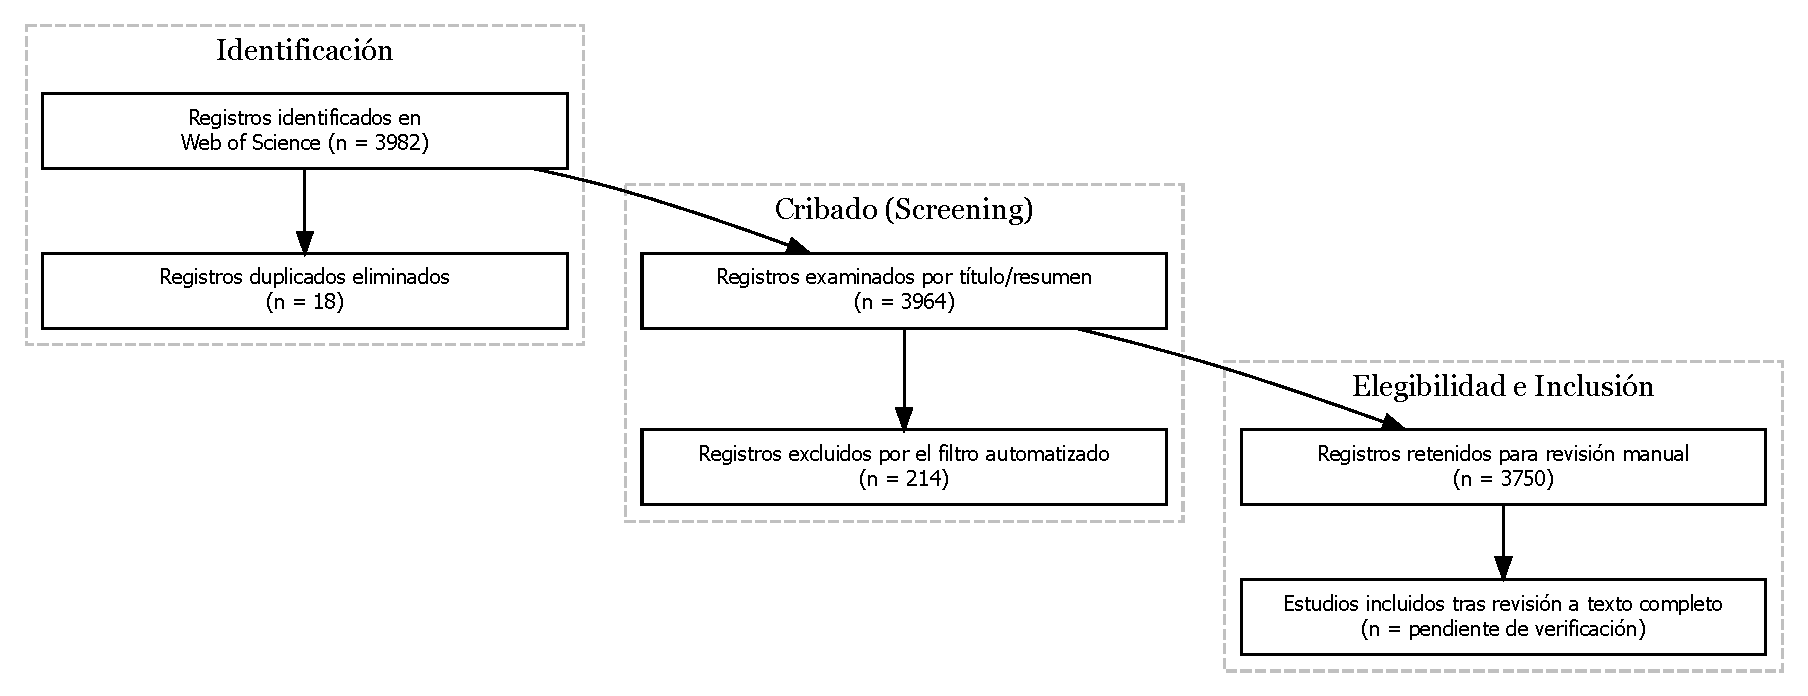
\includegraphics[width=1.0\textwidth]{../images/prisma-flowchart.pdf}
    \caption{Flujo preliminar de registros de WoS. Las cifras corresponden al procesamiento automatizado; la revisión manual y la inclusión final están pendientes.}
    \label{fig:prisma-flowchart}
\end{figure}